%\usepackage[top=2cm,bottom=2cm,left=1cm,right=1cm]{geometry}


\begin{titlepage}
     \begin{center}
	
\includegraphics[width=0.09\textwidth]{UNAM}\Large Universidad Nacional Autónoma de México
        	
\includegraphics[width=0.09\textwidth]{FI}\\[1cm]
        \Large Facultad de Ingeniería\\[1cm]
       % \Large División de Ciencias Básicas\\[1cm]
         \Large Laboratorio de Fundamentos de Control(6655)\\[1cm]
         %la clave antes era:4314
         \footnotesize Profesor: Salcedo Ubilla María Leonor Ing.\\[1cm]
        \footnotesize Semestre 2019-1\\[1cm]
        
       

        \Large Práctica No. 1\\[1cm]
        
           

\Large Introdcción MATLAB
        
         %Texto a la derecha
          \begin{flushright}
\footnotesize  Grupo 2\\[0.5cm]
\footnotesize Brigada: 4\\[0.5cm]
\footnotesize Rodrigo Adrián Martínez López\\[0.5cm]
\footnotesize Vivar Colina Pablo\\[0.5cm]
 \end{flushright}
    %Texto a la izquierda
          \begin{flushleft}
        \footnotesize Ciudad Universitaria Agosto de 2018.\\
          \end{flushleft}
         
          
        %\vfill
        %\today
   \end{center}
\end{titlepage}
 %agregar portada

\documentclass{article}
\usepackage[utf8]{inputenc}
\usepackage[spanish.mexico]{babel}

\title{Dispositivos}
\author{Pablo Vivar Colina}
\date{Septiembre 2017}

\usepackage{natbib}
\usepackage{graphicx}


%Circuitos
\usepackage{tikz}
\usepackage[american voltages, american currents,siunitx]{circuitikz}

%Plotting

\usepackage{pgfplots}
\pgfplotsset{width=10cm,compat=1.9} 
 %\usepgfplotslibrary{external}
\tikzexternalize 



\begin{document}


%\maketitle

%\usepackage[top=2cm,bottom=2cm,left=1cm,right=1cm]{geometry}


\begin{titlepage}
     \begin{center}
	
\includegraphics[width=0.09\textwidth]{UNAM}\Large Universidad Nacional Autónoma de México
        	
\includegraphics[width=0.09\textwidth]{FI}\\[1cm]
        \Large Facultad de Ingeniería\\[1cm]
       % \Large División de Ciencias Básicas\\[1cm]
         \Large Laboratorio de Fundamentos de Control(6655)\\[1cm]
         %la clave antes era:4314
         \footnotesize Profesor: Salcedo Ubilla María Leonor Ing.\\[1cm]
        \footnotesize Semestre 2019-1\\[1cm]
        
       

        \Large Práctica No. 1\\[1cm]
        
           

\Large Introdcción MATLAB
        
         %Texto a la derecha
          \begin{flushright}
\footnotesize  Grupo 2\\[0.5cm]
\footnotesize Brigada: 4\\[0.5cm]
\footnotesize Rodrigo Adrián Martínez López\\[0.5cm]
\footnotesize Vivar Colina Pablo\\[0.5cm]
 \end{flushright}
    %Texto a la izquierda
          \begin{flushleft}
        \footnotesize Ciudad Universitaria Agosto de 2018.\\
          \end{flushleft}
         
          
        %\vfill
        %\today
   \end{center}
\end{titlepage}
 %agregar portada

\section{Marco teórico}

\subsection{Rectificador de media onda}

El rectificador de media onda es un circuito empleado para eliminar la parte negativa o positiva de una señal de corriente alterna de lleno conducen cuando se polarizan inversamente. Además su voltaje es positivo.\citep{circuitoMediaOnda}

\begin{figure}[h!]
    \centering
    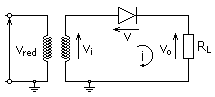
\includegraphics{Circuito_rectificador_media_onda.png}
    \caption{Caption}
    \label{fig:rectificadorMedia}
\end{figure}

\subsection{Rectificador de onda completa}

Un rectificador de onda completa es un circuito empleado para convertir una señal de corriente alterna de entrada (Vi) en corriente de salida (Vo) pulsante. A diferencia del rectificador de media onda, en este caso, la parte negativa de la señal se convierte en positiva o bien la parte positiva de la señal se convertirá en negativa, según se necesite una señal positiva o negativa de corriente continua.

Existen dos alternativas, bien empleando dos diodos o empleando cuatro (puente de Graetz).\citep{circuitoOnda}

\subsection{Tensión rectificada}

\begin{itemize}
    \item  Vo (corriente continua de salida) = Vi ( corriente alterna de entrada) = Vs/2 en el rectificador con diodos.
    \item  Vo = Vi = Vs en el rectificador con puente de Graetz.
\end{itemize}

   

Si consideramos la caída de tensión típica en los diodos en conducción, aproximadamente 0,7V; tendremos que para el caso del rectificador de doble onda la Vo = |Vi| - 1,4V.\citep{circuitoOnda}\\


\begin{figure}[h!]
    \centering
    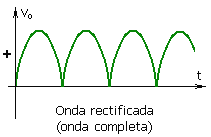
\includegraphics[scale=0.8]{OndaCompleta.png}
   % \caption{Onda Completa}
    \label{fig:my_label}
\end{figure}



\subsection{Rizado}

El rizado, algunas veces llamado fluctuación o ripple (del inglés), es el pequeño componente de alterna que queda tras rectificarse una señal a corriente continua. El rizado puede reducirse notablemente mediante un filtro de condensador, este proceso es llamado a veces "filtrar", y debe entenderse como la reducción a un valor mucho más pequeño de la componente alterna remanente tras la rectificación, pues, de no ser así, la señal resultante incluye un zumbido a 60 ó 50 Hz muy molesto, por ejemplo, en los equipos de audio.\citep{Rizado}\\

$(V_r)_{pp}$ es el voltaje de rizado de pico a pico. Recordar que $(V_r)_{pp}$ = $2\sqrt{2}(V_r)_{ef}$.\\

\begin{itemize}
    \item $I_L$es la corriente continua que demanda la carga.
    \item $f$ es la frecuencia del rizado. Esta frecuencia es igual a $f_{red}$ en un rectificador de media onda e igual a $2f_{red}$ en un rectificador de onda completa.
    \item $C$ es la capacidad del condensador.
\end{itemize}

El factor de rizado es un indicador de la efectividad del filtro y se define como:\\

\begin{equation}
     r = 100\left(\frac{V_r}{V_{cd}}\right) \quad \textrm{donde }
\end{equation}

Vr es el voltaje de rizado eficaz (rms, valor medio cuadrático)y Vcd es el valor de CD (corriente continua promedio) del voltaje de salida del filtro. Cuanto menor sea el factor de rizado, mejor será el filtro. El factor de rizado puede reducirse incrementando el valor del condensador del filtro.\citep{Rizado}\\

 \section{Material}

\begin{itemize}
    \item Resistores de distintos valores
    \item Condensadores de distintos valores
    \item 4 Diodos 1N4001
    \item Transformador de 12 [V] a 1 [A]
    
\end{itemize}

\section{Desarrollo}

\subsection{Circuito}


En la primera parte del experimento se usó el circuito que se muestra en la figura \ref{fig:rectificadorMediaO1} en el cual se midió la entrada del circuito (onda completa) y se registró la salida (espectro de media onda).\\

Para éste circuito se usó un transformado con tap central de 12 [V] a 1 [A].\\

\begin{figure}[ht!]
    \centering
    \begin{circuitikz}
    
        \draw (0,0) node [transformer](T){};
        \draw  (1,0) to[D,v=D](3,0);  
        \draw (3,0)to[C,l=C](3,-2.1)
        (1,-2.1)--(3,-2.1);
        \draw  (5,0) to[R,l=R](5,-2.1)
        (3,0)--(5,0)
        (3,-2.1)--(5,-2.1)
        ;
        
    \end{circuitikz}
    \caption{Rectificador media Onda}
    \label{fig:rectificadorMediaO1}
\end{figure}


\begin{table}[ht!]
\centering

\begin{tabular}{|c|c|c|c|c|c|}
\hline
Prueba & V rizo & V directa & V pico  & C        & R    \\ \hline
1      & 10V    & 10V       & 20V     & 10 uF    & 1k   \\ \hline
2      & 0V     & 15V       & 15V     & 1000 uF  & 1k   \\ \hline
3      & 20mV   & 15V       & 12.02V  & 1000 uF  & 10k  \\ \hline
4      & 2V     & 15V       & 17V     & 10 uF    & 10k  \\ \hline
5      & 15V    & 5V        & 20V     & 0.047uF  & 10k  \\ \hline
6      & 15V    & 5V        & 20V     & 0.047 uF & 100k \\ \hline
7      & 0.2V   & 15V       & 12.2V   & 10uF     & 100k \\ \hline
8      & 5mV    & 15V       & 15.005V & 1000 uF  & 100k \\ \hline
\end{tabular}

\caption{Registro de resultados}
\label{tablaSimple}
\end{table}

En la tabla\ref{tablaSimple} podemos apreciar los diferentes comportamientos del voltaje cambiando los componentes del circuito mostrado en la figura \ref{fig:rectificadorMediaO1}, los componentes que se fueron cambiando a lo largo de las pruebas fueron el capacitor y el resistor.\\

\subsection{Circuito}

\begin{figure}[ht!]
    \centering
    \begin{circuitikz}
    
        \draw (0,0) node [transformer](T){};
        \draw  (1,0) to[D,v=A](3,0); 
        \draw  (1,-2.1) to[D,v=B](3,-2.1)
        (3,-2.1)--(3,-1.3)
        (3,-1.3) arc (-90:90:0.25) 
        (3,0)--(3,-0.8)
        
        ; 
        
        \draw (4,0)to[C,l=C](4,-1.05)
        (3,0)--(6,0)
        (0,-1.05)--(6,-1.05)
        
       ;
        \draw  (5.5,0) to[R,l=R](5.5,-1.05)
        
        ;
        
    \end{circuitikz}
    \caption{Rectificador Onda Completa}
    \label{fig:rectificadorOndaCompleta}
\end{figure}


\begin{table}[ht!]
\centering
\begin{tabular}{|c|c|c|c|c|c|}
\hline
Prueba & V rizo       & V directa & V pico   & C       & R    \\ \hline
1      & 7V           & 5V        & 12V      & 0.047uF & 1k   \\ \hline
2      & 3V           & 6V        & 9V       & 10uF    & 1k   \\ \hline
3      & 50mV         & 6V        & 7V       & 1000uF  & 1k   \\ \hline
4      & 9mV          & 7V        & 7V       & 1000uF  & 1k   \\ \hline
5      & 0.5V         & 6V        & 6V       & 10uF    & 10k  \\ \hline
6      & 6.8V         & 4V        & 10.8V    & 0.047uF & 10k  \\ \hline
7      & 5V           & 5V        & 10V      & 0.047uF & 100k \\ \hline
8      & 0.5mV        & 7V        & 7.005V   & 0.057uF & 100k \\ \hline
9      & \textless5mV & 8V        & aprox 8V & 1000uF  & 100k \\ \hline
\end{tabular}


\caption{Registro de datos}
\label{datosRectificadorOC}
\end{table}

%######## AQUI VA LA PRACTICA ########

%mbi armiya naroda! :D
%https://www.youtube.com/watch?v=3D5-pleHkdk





\bibliographystyle{plain}
\bibliography{referencias8.bib}

\end{document}